\section{Correction for Dasgupta--Pal}
\label{chap:correction}
\subsection{Bitwise Description of the Dasgupta--Pal Cryptosystem}
The Dasgupta--Pal cryptosystem \cite{dasgupta_design_2016} encrypts each bit in a bit string independently.
In terms of the encryption of a single bit, the Dasgupta--Pal cryptosystem can be described as follows:
\begin{description}
	\item[Key generation]
	Let the secret key, $S_k$ be a large prime.
	Let the public refresh key, $R_k$, be $S_k \times z$, where $z$ is a large even integer.
	\item[Encryption]
	Given a message $m$, the encryption function is defined as
	\begin{align*}
		E(m) = m + S_kr
	\end{align*}
	where $r$ is a random integer.
	\item[Decryption]
	Given a ciphertext $c$, the decryption function is defined as
	\begin{align*}
		D(c) = c \bmod S_k \bmod 2
	\end{align*}
\end{description}
The homomorphic operations are then defined as
\begin{description}
	\item[\textsc{xor} on ciphertexts]
	\begin{align*}
		D(E(a)+E(b)) = a \textsc{ xor } b = (a + b) \bmod 2
	\end{align*}
	\item[\textsc{and} on ciphertexts]
	\begin{align*}
		D(E(a)\times E(b)) = a \textsc{ and } b = ab \bmod 2
	\end{align*}
\end{description}
After repeated operations on ciphertexts, the resulting ciphertext can grow in magnitude.
To prevent storage issues and keep the ciphertext size small, a refresh function is used.
\begin{description}
	\item[Refresh function]
	Given a ciphertext $c$, the refresh function is defined as
	\begin{align*}
		R(c) = c \bmod R_k
	\end{align*}
\end{description}
\subsection{Cases Where Decryption Fails}
We consider the following quantity:
\begin{align}
	\label{eq:cornercase_ciphertext}
	D(\underbrace{E(1)+E(1)+\cdots+E(1)}_{S_k \text{ times}}).
\end{align}
Since $S_k$ is odd, the corresponding operation in the plaintext space is
\begin{align*}
	\label{eq:cornercase_plaintext}
	\underbrace{1 \textsc{ xor } 1 \textsc{ xor } \cdots \textsc{ xor } 1}_{S_k \text{ times}} = 1.
\end{align*}
However, evaluating Equation \ref{eq:cornercase_ciphertext} yields:
\begin{align*}
	D(\underbrace{E(1)+E(1)+\cdots+E(1)}_{S_k \text{ times}})
	&= D\left(\sum_{i=1}^{S_k}{(1+S_kr_i)}\right)\\
	&= D\left(S_k + S_k\sum_{i=1}^{S_k}{r_i}\right)\\
	&= \left(S_k + S_k\sum_{i=1}^{S_k}{r_i}\right) \bmod S_k \bmod 2\\
	&= 0 \bmod 2\\
	&= 0.
\end{align*}
Since $\underbrace{1 \textsc{ xor } 1 \textsc{ xor } \cdots \textsc{ xor } 1}_{S_k \text{ times}} = 1\neq 0 = D(\underbrace{E(1)+E(1)+\cdots+E(1)}_{S_k \text{ times}})$, we have shown an instance where incorrect decryption occurs given a sequence of operations on ciphertexts.

\subsection{Proposed Correction and Proof of Correctness}
We now show that setting the secret key $S_k$ to $2p$, where $p$ is a prime, fixes the issue in the original cryptosystem.
\begin{theorem}
	Suppose $S_k = 2p$, where $p$ is a prime. Then when addition or multiplication is performed between any two ciphertexts, correct decryption is assured.
\end{theorem}
\begin{proof}
	Suppose $c_1, c_2$ are two ciphertexts such that
	\begin{align*}
		c_1 = a + S_kr_1\\
		c_2 = b + S_kr_2
	\end{align*}
	We first consider addition. We want to show that $(c_1+c_2)\bmod S_k$ has the same parity as $a+b$.
	By the division algorithm, we have $a+b = S_kq + r$, for some $q,r$, $q \geq 0, r > 0$. We can rewrite $c_1+c_2$ as
	\begin{align*}
		c_1+c_2 &= (a + S_kr_1) + (b + S_kr_2)\\
		&= (a+b)+ S_k(r_1 + r_2)\\
		&= (S_kq + r) + S_k(r_1 + r_2)\\
		&= r + S_k(q + r_1 + r_2).
	\end{align*}
	Therefore $(c_1+c_2)\bmod S_k = r$.
	It is enough to show that the parity of $a+b$ is the same as the parity of $r$. We consider cases based on the parity of $a+b$.
	\begin{description}
		\item[Case 1: $a+b$ is odd.]
			Since $a+b = S_kq + r$, $S_kq + r$ must also be odd.
			$S_k$ is even, so $S_kq$ is also even.
			For $S_kq + r$ to be odd, $r$ must be odd, since $S_k$ is even.

			Therefore, the parity of $a+b$ is the same as the parity of $r$.
		\item[Case 2: $a+b$ is even.]
			Since $a+b = S_kq + r$, $S_kq + r$ must also be even.
			$S_k$ is even, so $S_kq$ is also even. For $S_kq + r$ to be even, $r$ must be even , since $S_k$ is even.

			Therefore, the parity of $a+b$ is the same as the parity of $r$.
	\end{description}
	Therefore correct decryption is assured for the sum of ciphertexts.

	We now consider multiplication. We want to show that $c_1c_2 \bmod S_k$ has the same parity as $ab$. Similar to the addition case, by the division algorithm, we can write $ab = S_kq + r$, $q > 0, r > 0$ for some $q,r$. We can rewrite $c_1c_2$ as
	\begin{align*}
		c_1c_2 &= (a + S_kr_1) \times (b + S_kr_2)\\
		&= ab + S_k(br_1 + ar_2 + S_kr_1r_2)\\
		&= (S_kq + r) + S_k(br_1 + ar_2 + S_kr_1r_2)\\
		&= r + S_k(q + br_1 + ar_2 + S_kr_1r_2).
	\end{align*}
	Therefore $c_1c_2 \bmod S_k = r$.
	It is enough to show that the parity of $ab$ is the same as the parity of $r$. We consider cases based on the parity of $ab$.
	\begin{description}
		\item[Case 1: $ab$ is odd.]
			Since $ab = S_kq + r$, $S_kq + r$ must also be odd.
			$S_k$ is even, so $S_kq$ is also even.
			For $S_kq + r$ to be odd, $r$ must be odd, since $S_k$ is even.

			Therefore, the parity of $a+b$ is the same as the parity of $r$.
		\item[Case 2: $ab$ is even.]
			Since $ab = S_kq + r$, $S_kq + r$ must also be even.
			$S_k$ is even, so $S_kq$ is also even. For $S_kq + r$ to be even, $r$ must be even, since $S_k$ is even.

			Therefore, the parity of $ab$ is the same as the parity of $r$.
	\end{description}
	Therefore, correct decryption is assured for both addition and multiplication of ciphertexts.
\end{proof}



\section{Numerical Approximations}
\newcommand*\diff{\mathop{}\!\mathrm{d}}

Transcendental functions such as the exponential and logarithmic functions are usually implemented in computer hardware and software libraries using minimax polynomials, which are determined numerically using the Remez algorithm \cite{harrison_computation_1999}.
However, the Remez algorithm relies on iteratively refining the polynomial coefficients, which requires knowledge of the argument passed to the transcendental function.

We cannot directly apply this approach in privacy-preserving image processing as we do not have knowledge of the exact value of the function arguments. In order to calculate a function under a  homomorphic cryptosystem, it is necessary to express the function in terms of the homomorphic operations.
In this section, we discuss approximations for the logarithm ($\log(1+x)$) and power ($x^r$) functions using only addition, subtraction, multiplication, and division operations.

\subsection{Approximation for $\log(1+x)$}
\label{sec:logapproximation}
We approximate the function $f(x)=\log(1+x)$ using a similar method to that described in
\cite{khattri_new_2009}.
We let $x = 1/n$ and consider the integral
\begin{equation}
	\label{eq:log_integral}
  	\int_{n}^{n+1}{\frac{1}{x}\diff x}=\log{\left(1+\frac{1}{n}\right)}.
\end{equation}

This integral can be approximated using the five-point Gauss-Legendre quadrature rule \cite{kythe_quadrature_2002}. We first convert the integral to an integral over the interval $[-1,1]$ using the following transformation:
\begin{align*}
	\int_a^b{f(x)\diff x}
	&= \frac{b-a}{2}\int_{-1}^{1}{f\left(\frac{b-a}{2}x+\frac{a+b}{2}\right)\diff x}.
\end{align*}
Then, we approximate the integral using the following summation:
\begin{align*}
  \int_{-1}^{1}{f(x)\diff x} &= \sum_{i=1}^{5}{w_if(x_i)},
\end{align*}
where
\begin{multicols}{2}
	\noindent
	\begin{align*}
		w_1 &= 0\\
		w_2 &= \frac{1}{21}\sqrt{245-14\sqrt{70}}\\
		w_3 &= -\frac{1}{21}\sqrt{245-14\sqrt{70}}\\
		w_4 &= \frac{1}{21}\sqrt{245+14\sqrt{70}}\\
		w_5 &= -\frac{1}{21}\sqrt{245+14\sqrt{70}}
	\end{align*}
	\columnbreak
	\begin{align*}
		x_1 &= \frac{128}{225}\\
		x_2 &= \frac{1}{900}\left( 322 + 13\sqrt{70}\right)\\
		x_3 &= \frac{1}{900}\left( 322 + 13\sqrt{70}\right)\\
		x_4 &= \frac{1}{900}\left( 322 - 13\sqrt{70}\right)\\
		x_5 &= \frac{1}{900}\left( 322 - 13\sqrt{70}\right)
	\end{align*}
\end{multicols}
Applying this procedure to the integral in equation \ref{eq:log_integral} using SageMath 8.3 yields the following approximation:
\begin{equation}\label{eq:standardquadrature}
  \log(1+x) \approx
  \frac{137x^5 + 2310x^4 + 9870x^3 + 15120x^2 + 7560x}
  {30x^5 + 900x^4 + 6300x^3 + 16800x^2 + 18900x + 7560}.
\end{equation}

While the closed form approximation in equation \ref{eq:standardquadrature} is accurate for values of $x$ near zero, it diverges from $\log{(1+x)}$ significantly for large values of $x$, as shown in figure \ref{fig:standardquadrature}.
\begin{figure}[!ht]
    \centering
    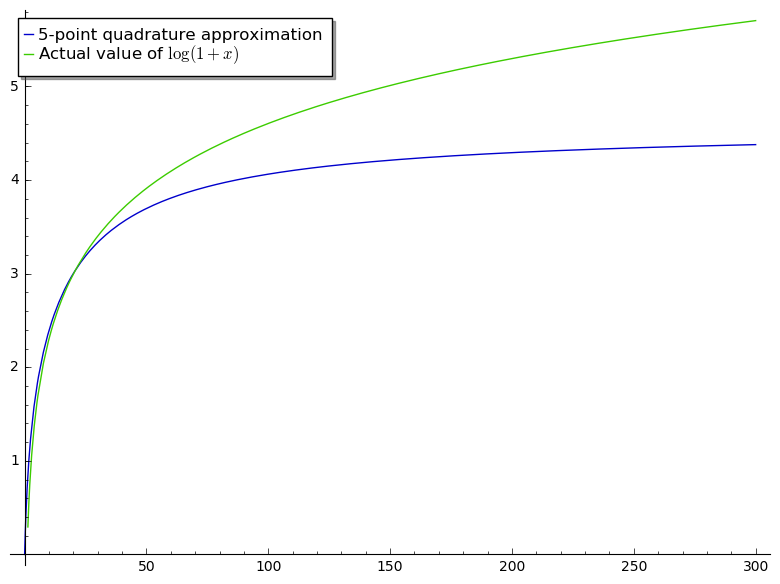
\includegraphics[width=.8\linewidth]{figures/StandardQuadrature.png}
    \caption{Graph of $\log{(1+x)}$ and the approximation in equation \ref{eq:standardquadrature}}
    \label{fig:standardquadrature}
\end{figure}

As we only need accuracy for arguments $x \in [0, 255]$, we can scale the approximation by a constant factor $\alpha$ as follows:
\begin{align*}
  \log{(1+x)} &= \log{\left(\frac{\alpha + \alpha x}{\alpha}\right)}\\
  &= \log{(\alpha + \alpha x)} - \log{\alpha}\\
  &= \log{\left(\alpha+\frac{\alpha}{n}\right)} - \log{\alpha}\\
  &= \log{\left(\frac{\alpha n + \alpha}{n}\right)} - \log{\alpha}\\
  &= \int_{n}^{\alpha n + \alpha}{\frac{1}{x}\diff x} - \log{\alpha}
\end{align*}

Applying the five-point Gauss-Legendre quadrature rule with $\alpha = 1/20$ using SageMath 8.3, we arrive at the approximation:
\begin{align}\label{eq:scaledquadrature}
  \begin{split}
    &\log(1+x) \\
    &\approx \frac{137x^5 + 33185x^4 + 931370x^3 - 13403630x^2 - 289469315x - 713567363}
    {30(x^5 + 505x^4 + 42010x^3 + 923010x^2 + 5722005x + 8040501)} \\
    &+ \log{20}
  \end{split}
\end{align}

Figure \ref{fig:scaledquadrature} is a graph of the absolute error of the scaled approximation and the exact value of $\log{(1+x)}$. Using SageMath 8.3, it was numerically determined that the maximum absolute error of this approximation in the range $x\in[0,255]$ is approximately $0.0103315865985758$, occurring at $x=255$. This is an improvement from the approximation in equation \ref{eq:standardquadrature}, which has a maximum absolute error of $1.19717868468392$, similarly occurring at $x=255$.

\begin{figure}[h]
    \centering
    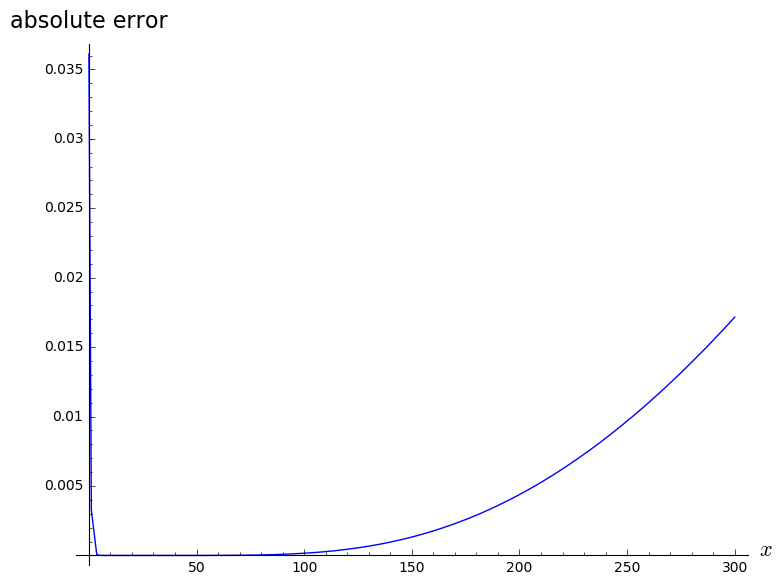
\includegraphics[width=.9\linewidth]{figures/ModifiedQuadratureAbsoluteError.png}
    \caption{Graph of the absolute error of $\log{(1+x)}$ and the approximation in equation \ref{eq:scaledquadrature}}
    \label{fig:scaledquadrature}
\end{figure}

\subsection{Approximation for $x^\gamma$}
To approximate $x^\gamma$ for any $\gamma \in \mathbb{R}$, we rewrite $x^\gamma$ as follows:
\begin{align*}
  x^\gamma = e^{\log{x^\gamma}} = e^{\gamma\log{x}}.
\end{align*}

This expression can then be approximated using the Maclaurin series expansion for $e^x$, which converges for all $x$.
\begin{align*}
  e^x &= \sum_{n=0}^{\infty}{\frac{x^n}{n!}}\\
  \Rightarrow e^{\gamma\log{x}} &= \sum_{n=0}^{\infty}{\frac{(\gamma\log{x})^n}{n!}}
\end{align*}

As we already have an approximation for the natural logarithm, we can evaluate partial sums of the above infinite series to arrive at approximations for $x^\gamma$.